\documentclass[twoside,11pt]{article}

% Any additional packages needed should be included after jmlr2e.
% Note that jmlr2e.sty includes epsfig, amssymb, natbib and graphicx,
% and defines many common macros, such as 'proof' and 'example'.
%
% It also sets the bibliographystyle to plainnat; for more information on
% natbib citation styles, see the natbib documentation, a copy of which
% is archived at http://www.jmlr.org/format/natbib.pdf

\usepackage{jmlr2e}
\usepackage{amsmath}
\usepackage{enumitem}
\usepackage{subcaption}

% Definitions of handy macros can go here

\newcommand{\dataset}{{\cal D}}
\newcommand{\fracpartial}[2]{\frac{\partial #1}{\partial  #2}}

% Heading arguments are {volume}{year}{pages}{submitted}{published}{author-full-names}

%\jmlrheading{1}{2000}{1-48}{4/00}{10/00}{Marina Meil\u{a} and Michael I. Jordan}

% Short headings should be running head and authors last names

%\ShortHeadings{Ensemble Methods for Robust Feature Selection}{Meil\u{a} and Jordan}
\firstpageno{1}

\begin{document}

\title{Ensemble Methods for Robust Feature Selection}

\author{\name Benjamin Rapier \email benjamin.rabier@campus.tu-berlin.de \\
       \addr Neural Information Processing Group\\
       Technical University Berlin\\
       10623 Berlin, Germany
       \AND
       \name Alexander Goscinski \email a.goscinski@mail.tu-berlin.de \\
       \addr Neural Information Processing Group\\
       Technical University Berlin\\
       10623 Berlin, Germany}

\editor{No Editor}

\maketitle

\begin{abstract}%   <- trailing '%' for backward compatibility of .sty file
  Abstract
\end{abstract}

\begin{keywords}
  Ensemble Methods, Robust, 
\end{keywords}

\section{Introduction}

Feature selection is a preprocessing step used in machine learning application to find a small subset of features in order to build a more accurate, simpler and faster model. Moreover it allows domain experts to gain a better understanding of the data, by focusing on the selected subset. However, in domains such as biomedical applications subsequent analysis are costly. Therefore not only the model performance but also the robustness of the feature selection method is important. Domain experts would prefer a more stable algorithm to have more confidence in the selected features. One approach for more robust results are ensemble methods.

Used in Machine Learning and Statistics, ensemble methods combine multiple algorithms in order to obtain better performance. The bagging method, which consists of using the same algorithm on multiple subsets, has already been studied \cite{saeys2008}. The method improved considerably the robustness of the feature selection algorithm and the model performance was not significantly degraded in most cases. The purpose of this paper is to investigate the effect of ensemble methods further by combining different feature selection methods.

\section{Feature selection methods}

Symmetrical Uncertainty (SU) \citep{press1996numerical} is entropy based measurement. It is the normalized mutual information between the feature and the class. The mutual information measures the influence of the knowledge of the class on the feature value in terms of entropy and normalizes it. More details about mutual information can be found in \cite{paninski2003estimation}.
\begin{equation}
  \label{eq:su}
  SU(F,C) = 2 \frac{H(F) - H(F|C)}{H(F) + H(C)} \textrm{, where } H(\cdot) \textrm{ is the entropy.}
\end{equation}

The second feature selection is RELIEFF \citep{kononenko1997overcoming}. For each sample $x_i$ the k nearest neighboring samples, using the $L_1$ norm, belonging the same class $\{\textrm{Near-hit}_{i, j}\}_{j=1..k}$ and the ones of the opposite class $\{\textrm{Near-miss}_{i, j}\}_{j=1..k}$ are selected. Then the difference is taken to update the weight vector representing how well each feature distinguishes samples of the two classes, as can be seen in equation \ref{eq:relief}. In all the experiments k was set to 5, which, empirically, gives satisfactory results.
\begin{equation}
  \label{eq:relief}
  W_i = W_i - \frac{1}{k}\sum_{j=1}^{k}|x_i - \textrm{Near-hit}_{i,j}| + \frac{1}{k}\sum_{j=1}^{k} |x_i - \textrm{Near-miss}_{i,j}|
\end{equation}

The third feature selection method used is a recursive feature elimination (RFE) with SVM \citep{guyon2002gene}. Recursive feature elimination fits a classifier and ranks the feature according to their importance in the model. In the case of the SVM, it is based on the weight vector of the hyperplane. More precisely after obtaining the solution for the primal problem of the SVM in equation \ref{eq:svm_primal}, the ranking coefficients $c_i$ for the features are then calculated by squaring the weights $c_i = w_i^2$.
\begin{alignat}{-1}
     \min_{w,b}  & \quad \frac12\|w\|^2 + C\sum_{i=1}^m \xi_i & & & \label{eq:svm_primal} \\ 
   \text{s.\,t.} & \quad y^{(i)} (w^Tx^{(i)} + b) & \quad \geq & \quad 1 -\xi_i &&
                   \quad \forall \, i = 1, \ldots, m \nonumber \\
                 & \quad \xi_i                  & \quad \geq & \quad 0 &&
                   \quad \forall \, i = 1, \ldots, m \nonumber 
\end{alignat}

The worst ranked features are then discarded and the procedure is repeated until only a subset of features is left. In the experiments, $10\%$ of the size of all the remaining features were discarded at each step. This means that. The procedure was repeated until a subset of the size of $1\%$ of all features was left.

The last feature feature selection method used is a RFE with Lasso.

\begin{equation}
  \min_w \quad \frac1{2 \, \textrm{\#features}} \, \|y - Xw\|^2_2 + \alpha \, \|w\|_1
\end{equation}


\section{Ensemble methods}

Ensemble

The different feature selection methods give as output a weight vector representing how well each feature distinguishes samples of the two classes. Those are then be combined by the ensemble method. Since different methods do not always have the same weight range, they are normalized to the range $[0,1]$. Moreover for the methods which can only rank data, such as methods based on RFE, their ranking are considered as weights, and so subsequently normalized the same way. 

Those normalized weights are combined using different techniques. The methods used in this paper can be grouped in three distinct categories: 

\begin{description}[align=left]
\item [Linear aggregation :] The average of the weights was taken as the new weight. Two version were used, one where a normalization of the weight sum is applied and the other without it.
\item [Non-linear aggregation :] To emphasize features with importance, the weights are non-linearly transformed with the equation \ref{eq:em_non_linear}. $\arctan$ in in combination with $\exp$ to considerably shrink the low weights. Finally the weights sum is normalized.

\begin{equation}
  \label{eq:em_non_linear}
  W_i = \frac{f \left( W_i \right)}{\sum_k f \left( W_k \right)} \quad with \quad f : x \rightarrow \exp( \arctan(x - 1) )
\end{equation}

\item [Performance related aggregation :] For each feature selector the best 1\% of the features were selected and used to measure the classification performance for multiple classifiers. The feature selection methods result were weighted accordingly to their accuracy. It was used in combination with the precedent ensemble methods.
\end{description}

Furthermore, different combinations of feature selectors were used in order to find combinations which work better than others.

\section{Evaluation}

While the purpose of this paper is to find a robust feature selection method, it is also necessary to evaluate the classification performance as domain expert have no interest in badly performing model. Hence those two aspects are always considered in combination.

\subsection{Data Sets}
Datasets are taken from the NIPS 2003 challenge (\cite{NIPS}). However, due to computation power constraints, not the whole dataset is always used. Additionally the colon data set (\cite{alon1999broad}) is used. Finally artificial data is also generated, since it is possible to control which features are meaningful. 

\begin{center}
    \begin{tabular}{| r | c | c | c | c | c |}
    \hline
    Name & \# Samples & \# Features & \# Class 1 & \# Class 2 & Ref\\ \hline
    Arcene & 200 & 10 000 & 112 & 88 & \cite{NIPS} \\
    Dexter & 600 & 20 000 & 300 & 300 & \cite{NIPS} \\
    Gisette & 200 & 5000 & 92 & 108 & \cite{NIPS} \\
    Colon & 62 & 2000 & 40 & 22 &  \cite{alon1999broad} \\
    Artificial & 300 & 10 000 & 150 & 150 & \\
    \hline
    \end{tabular}
\end{center}

The features of the artificial dataset are generated with two Gaussian distributions, depending on whether they are used in the labeling process or not.

\begin{align}
f \sim0.5 * \left[ N(0, 1) + N(0, \Sigma) \right]  \quad \text{with} \quad \Sigma_{ij} \sim U(0,1)
\end{align}
% \text{unsignificant} \quad & f \sim 0.5 * \left[ N(0, 1) + U(-1,1) \right]

To generate balanced binary labels, the significant features are first summed, then the median of the sums is subtracted, finally the sign is taken. 





\subsection{Experiments}

Feature selectors needs to be robust but also accurate, therefore both model performance and robustness were measured.

The model performance is estimated by measuring the balanced error rate of a set of classifiers: Lasso, linear SVM, k-nearest neighbor, Random Forest. For each classifier the performance was assessed using a 10-fold cross validation setting and trained on the best 1\% of the data.

To measure the robustness, different equally sized subsamples are drawn from the dataset. The feature selector runs on all of them, and the best ones are taken based. The subsets are then compared with a similarity measure. Given that the model performance is measured on the best 1\% of the features, the order of the feature should not be of importance but only if one is or not part of the best subset. Hence the Jaccard Index was used because only how many features are common to both sets is important for this measure. For two subsets of features $F_i$ and $F_j$ it is defined as:

\begin{equation}
J(F_i, F_j) = \frac{| F_i \cap F_j |}{| F_i \cup F_j |}
\end{equation}

\begin{figure}[!t]
\centering
\begin{subfigure}{.5\textwidth}
  \centering
  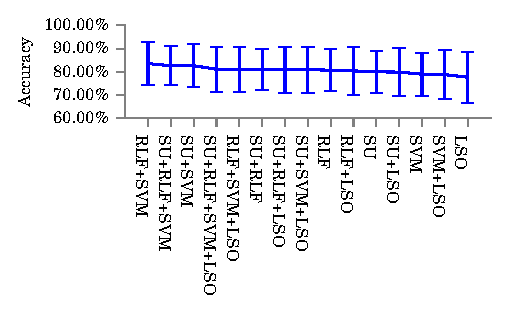
\includegraphics[width=1.07\textwidth]{images/Accuracy_of_the_different_combinations.pdf}
  \caption{Accuracy}
  \label{fig:combination_accuracy}
\end{subfigure}%
\begin{subfigure}{.5\textwidth}
  \centering
  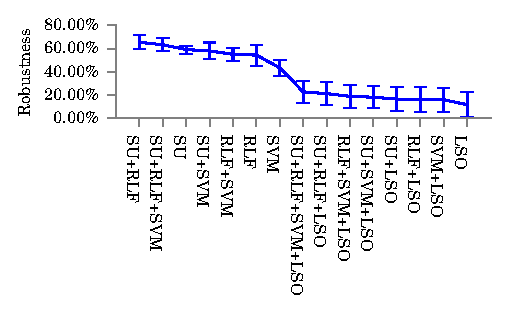
\includegraphics[width=1.07\textwidth]{images/Robustness_of_the_different_combinations.pdf}
  \caption{Robustness}
  \label{fig:combination_robustness}
\end{subfigure}
\caption{Results for the different combination of feature selectors. RLF and LSO corresponds respectively to RELIEFF and Lasso.}
\label{fig:combination_results}
\end{figure}

\begin{figure}[!t]
\centering
\begin{subfigure}{.5\textwidth}
  \centering
  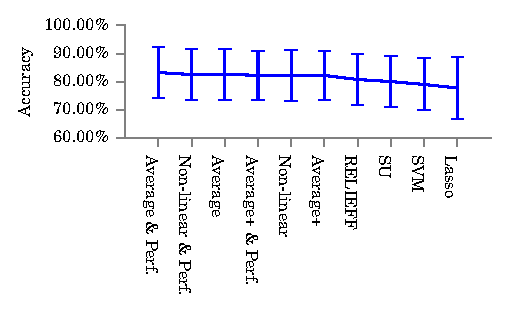
\includegraphics[width=1.07\textwidth]{images/Accuracy_of_the_different_methods.pdf}
  \caption{Accuracy}
  \label{fig:methods_accuracy}
\end{subfigure}%
\begin{subfigure}{.5\textwidth}
  \centering
  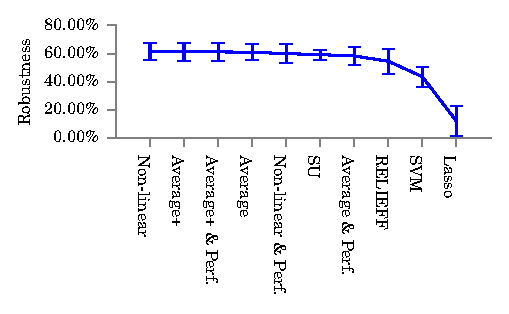
\includegraphics[width=1.07\textwidth]{images/Robustness_of_the_different_methods.pdf}
  \caption{Robustness}
  \label{fig:methods_robustness}
\end{subfigure}
\caption{Results for the different methods on average on the different combinations. "Average +" is the average method with the normalized sum. When "\& Perf." is indicated the performance was also used to aggregate the weights.}
\label{fig:methods_results}
\end{figure}


\subsection{Results}
In this section we present our results for the experiments
\subsubsection{Distribution of feature selectors}
\begin{figure}[h!]
  \centering
    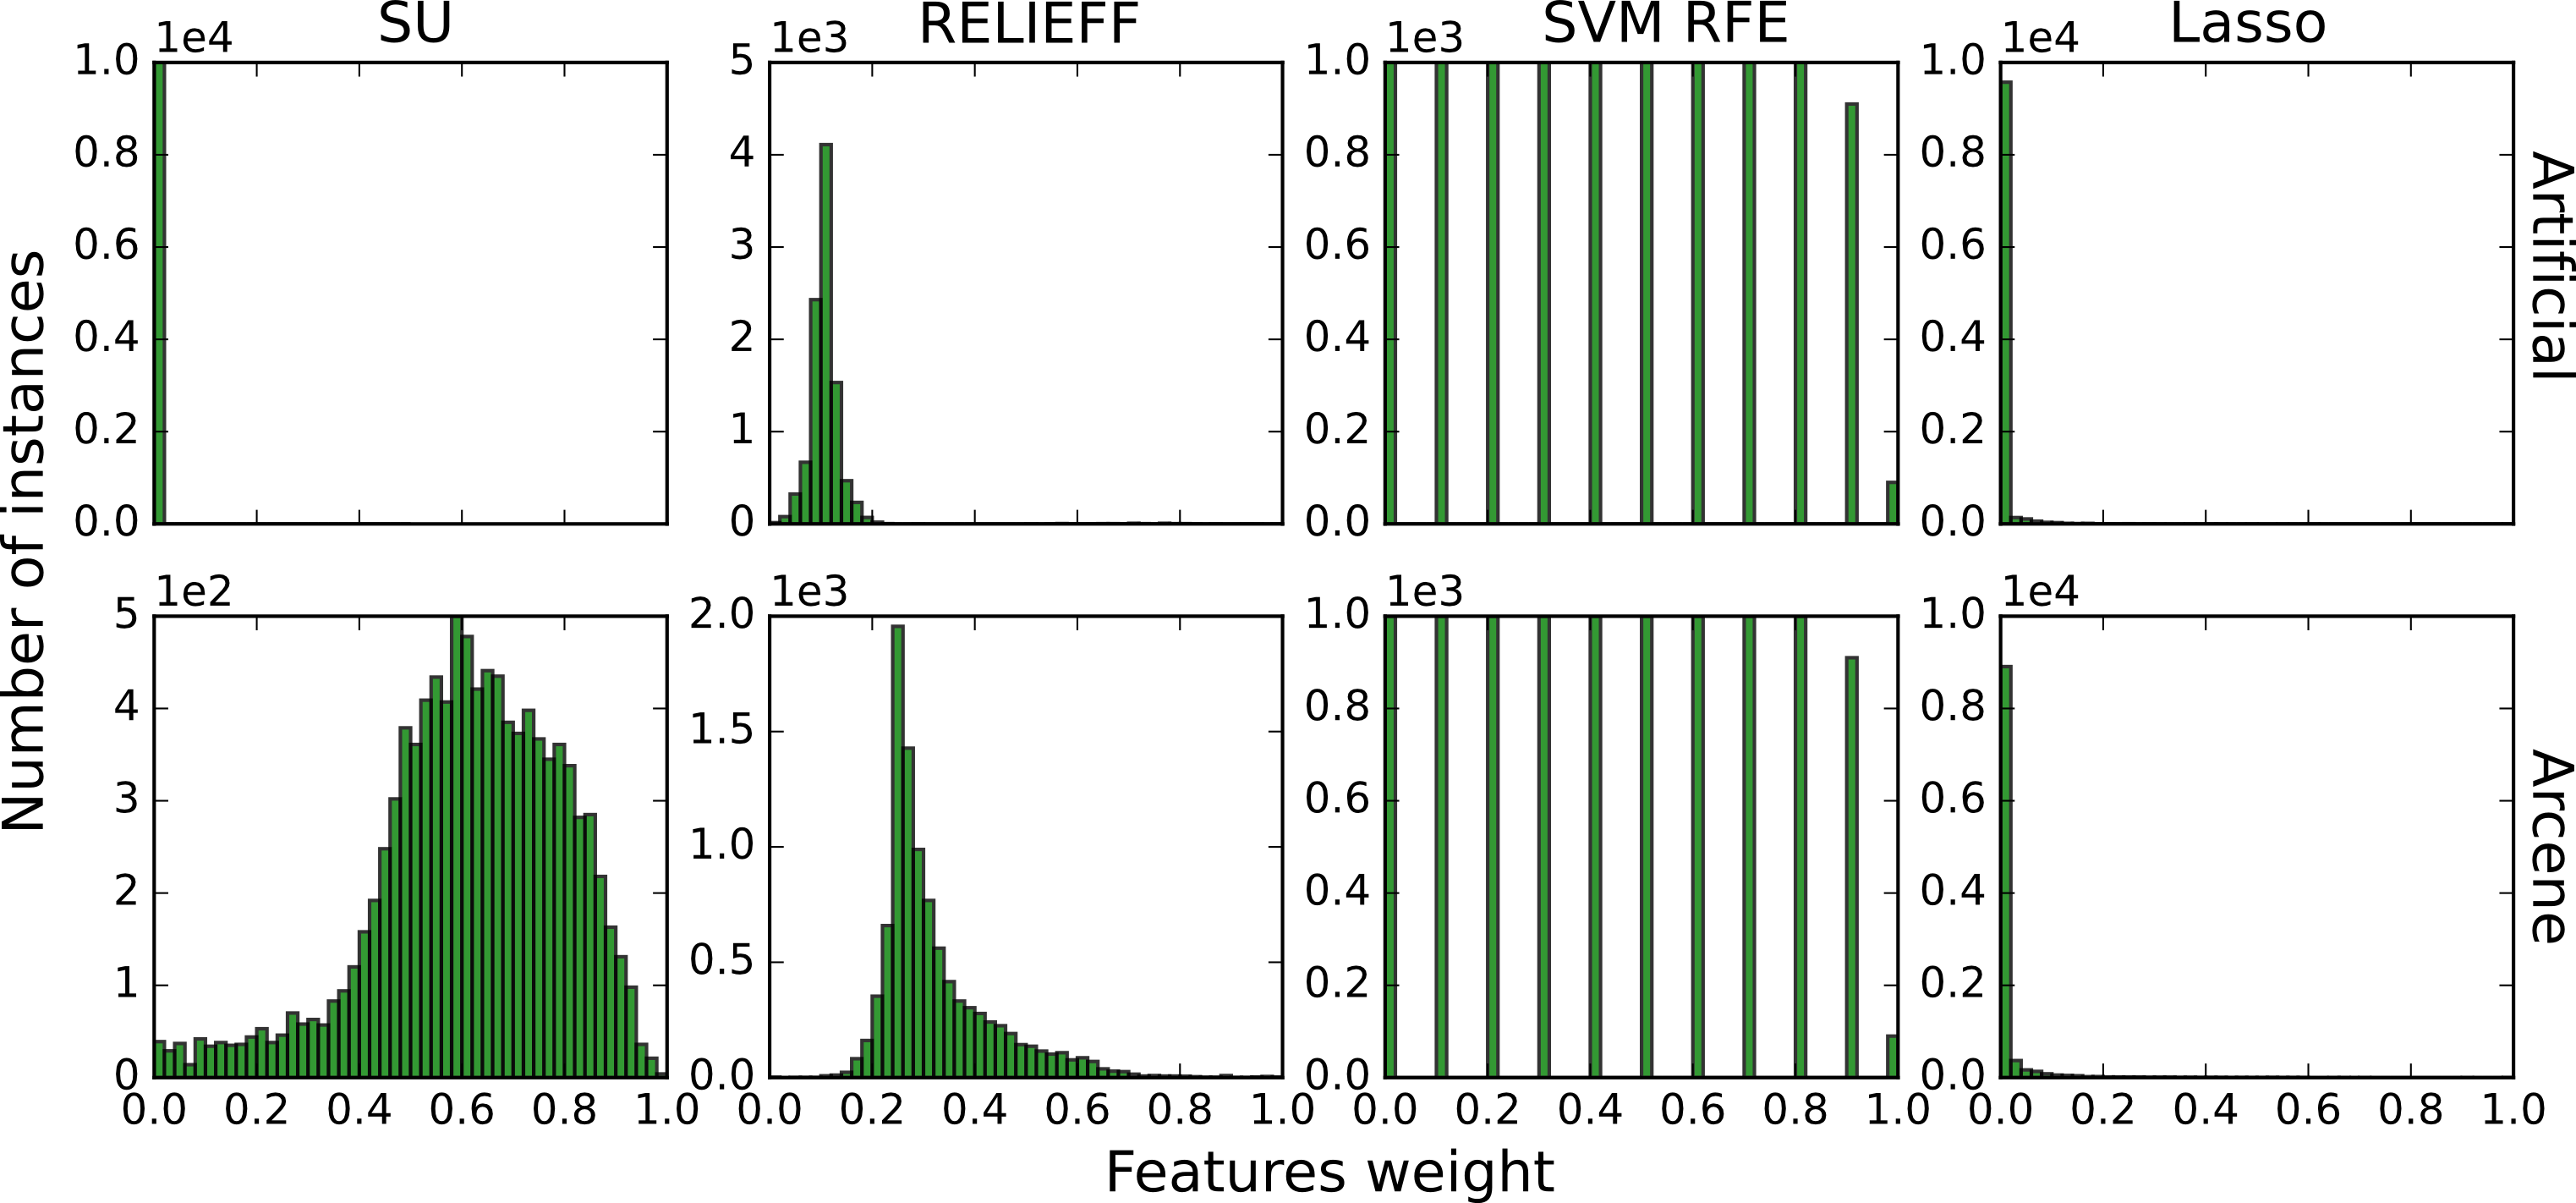
\includegraphics[width=\textwidth]{feature_weights_hist_arcene_artificial.png}
  \caption{The histograms of the feature weights for all used feature selectors on the arcene and artificial data set.}
  \label{fig:feature_weights_hist_arcene_artificial}
\end{figure}
In figure \ref{fig:feature_weights_hist_arcene_artificial} the histograms of the features weight can be seen for the arcene and the artificial data set. It is observable that the distribution of the feature weights have similiar shapes on each data set for RELIEFF, SVM RFE, Lasso logistic regression. In addition the distributions are centered around the same area. RELIEFF and Lasso seem to always have a strong peak. Lasso even stronger than RELIEFF, which is an effect of the sparsity of Lasso. On the other hand SU varies a lot on different data sets and does not seem to have a consistent shape. For some data sets like the artifical data set SU mainly outputs one value for all features. On others like arcene it is greatly distributed. The histograms for all data sets can be seen in the appendix in figure \ref{fig:feature_weights_hist}.

\subsubsection{Results for the artificial data set}
\begin{figure}
  \centering 
  \begin{subfigure}[b]{0.48\textwidth}
      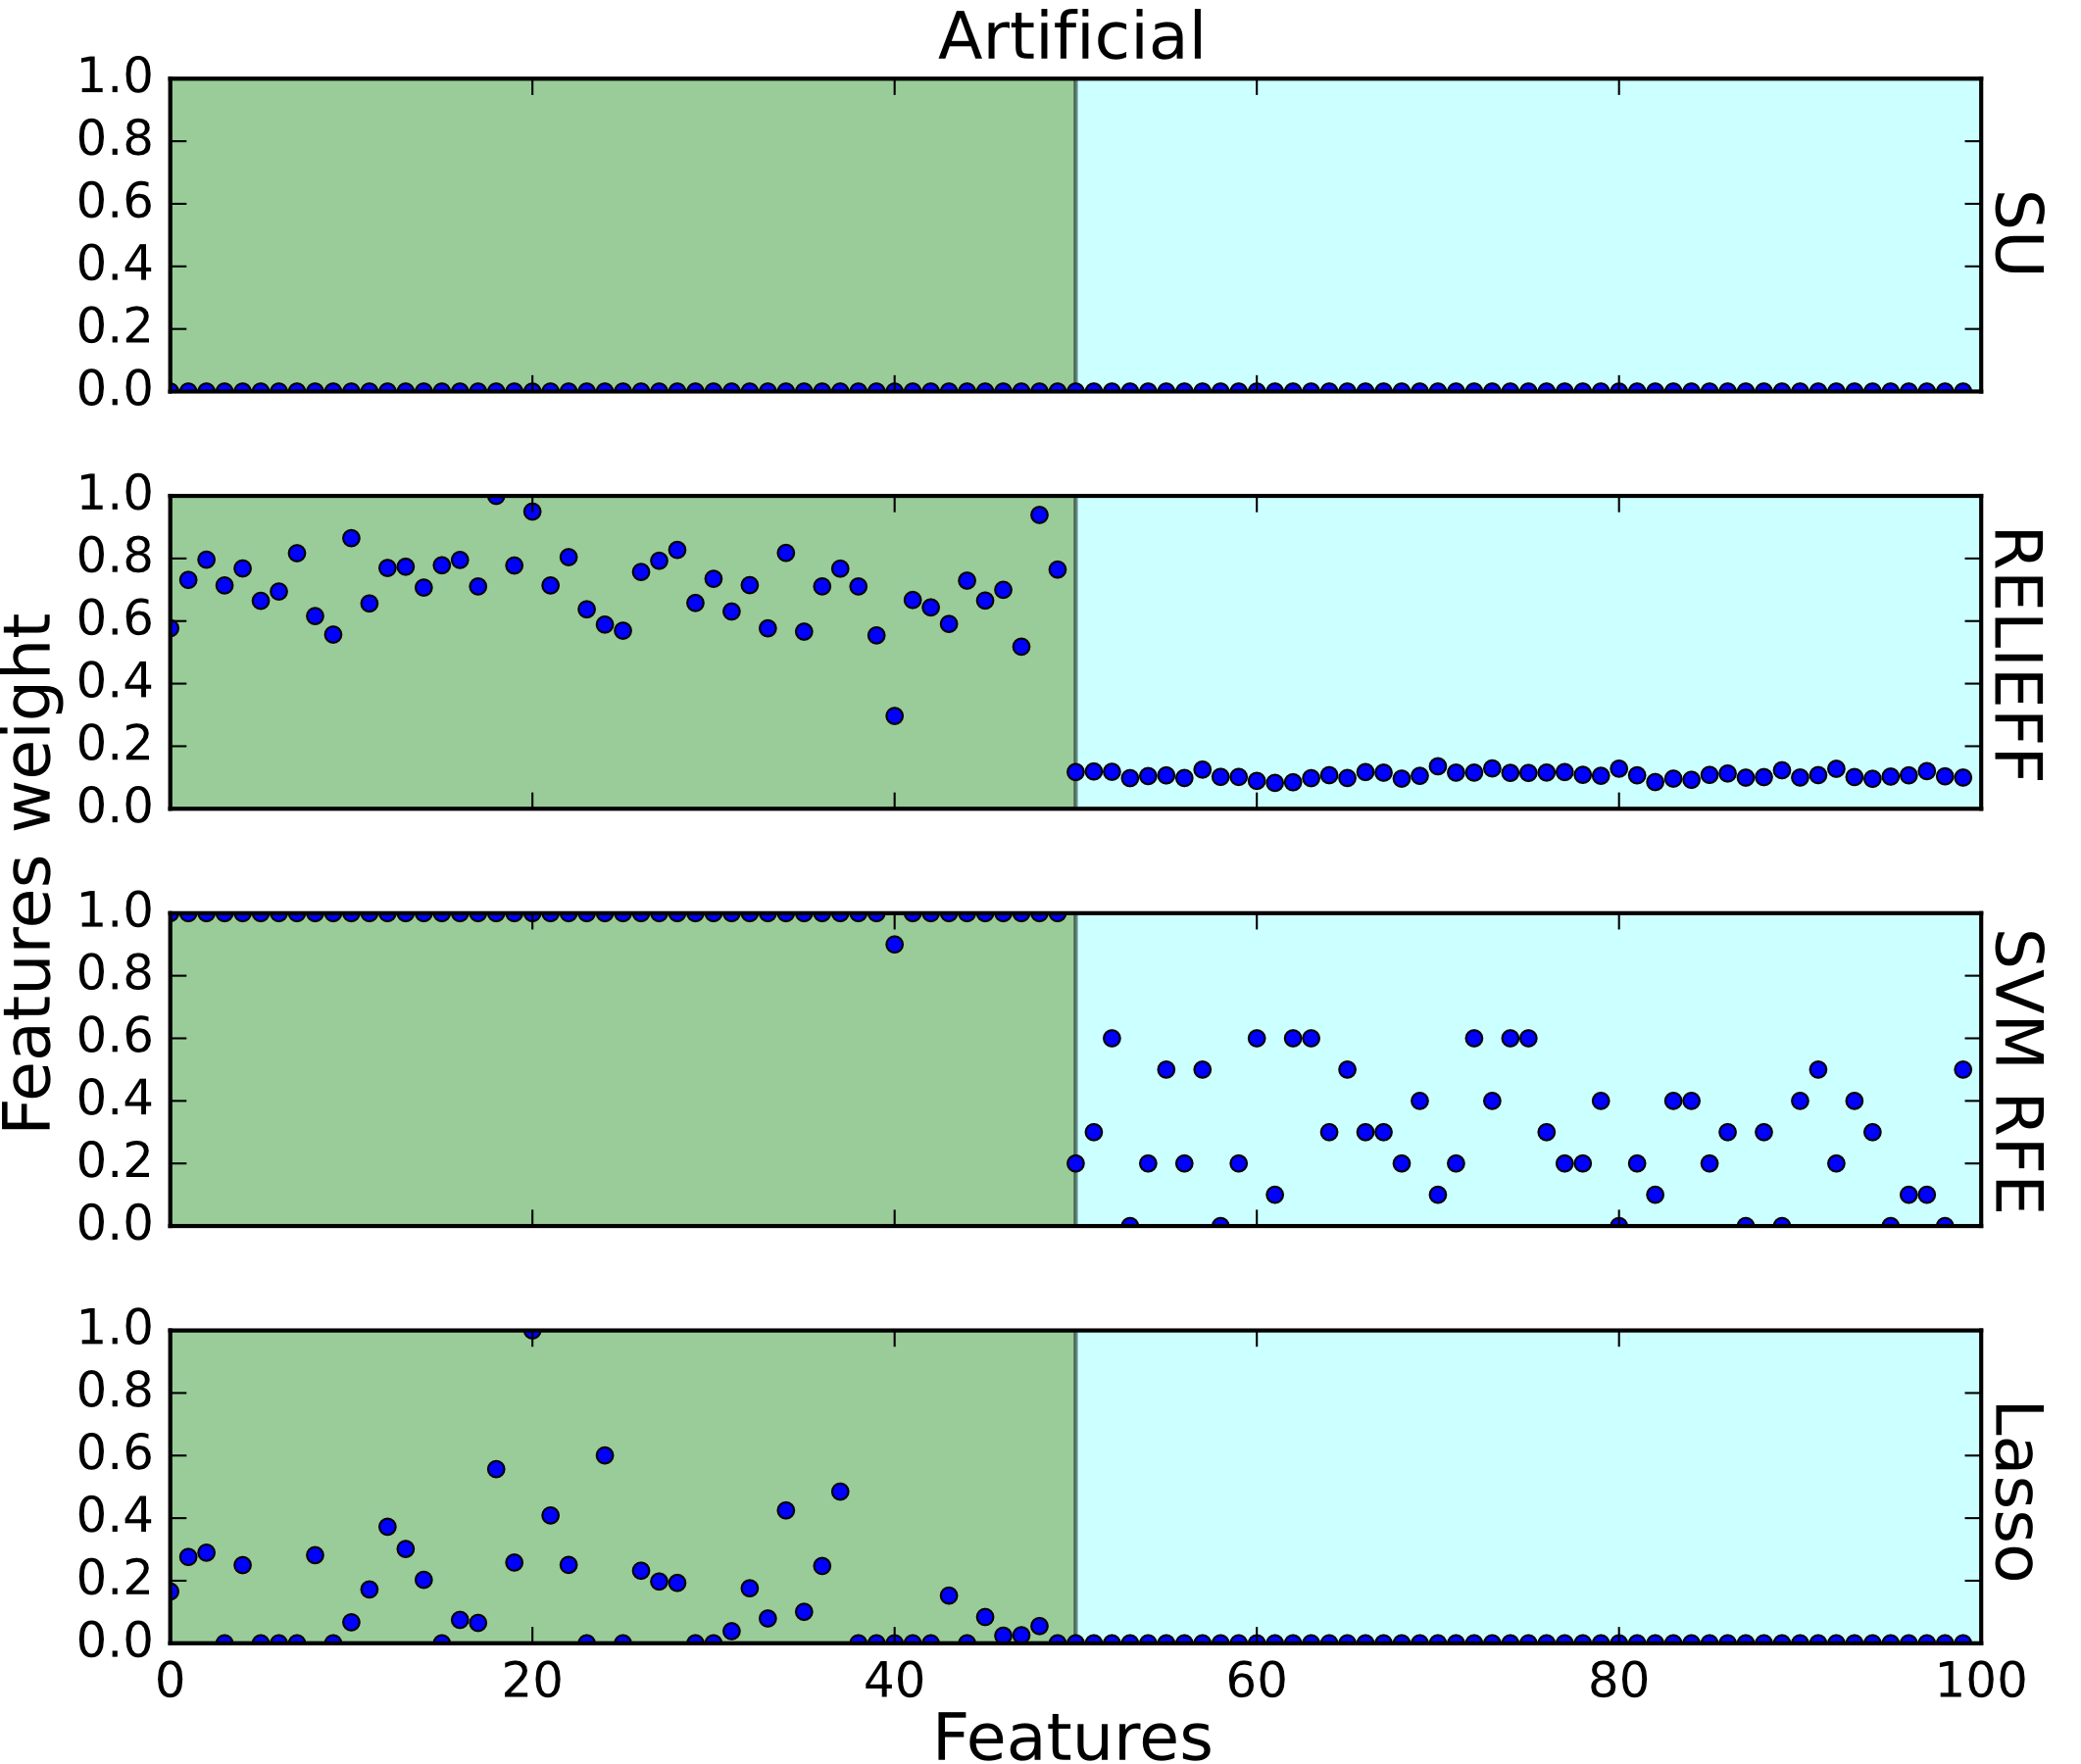
\includegraphics[width=\textwidth]{feature_weights_plot_artificial_only_features.png}
      \caption{Features weights for the real features.}
      \label{fig:feature_weights_plot_artificial_only_features}
  \end{subfigure}
  ~
  \begin{subfigure}[b]{0.48\textwidth}
    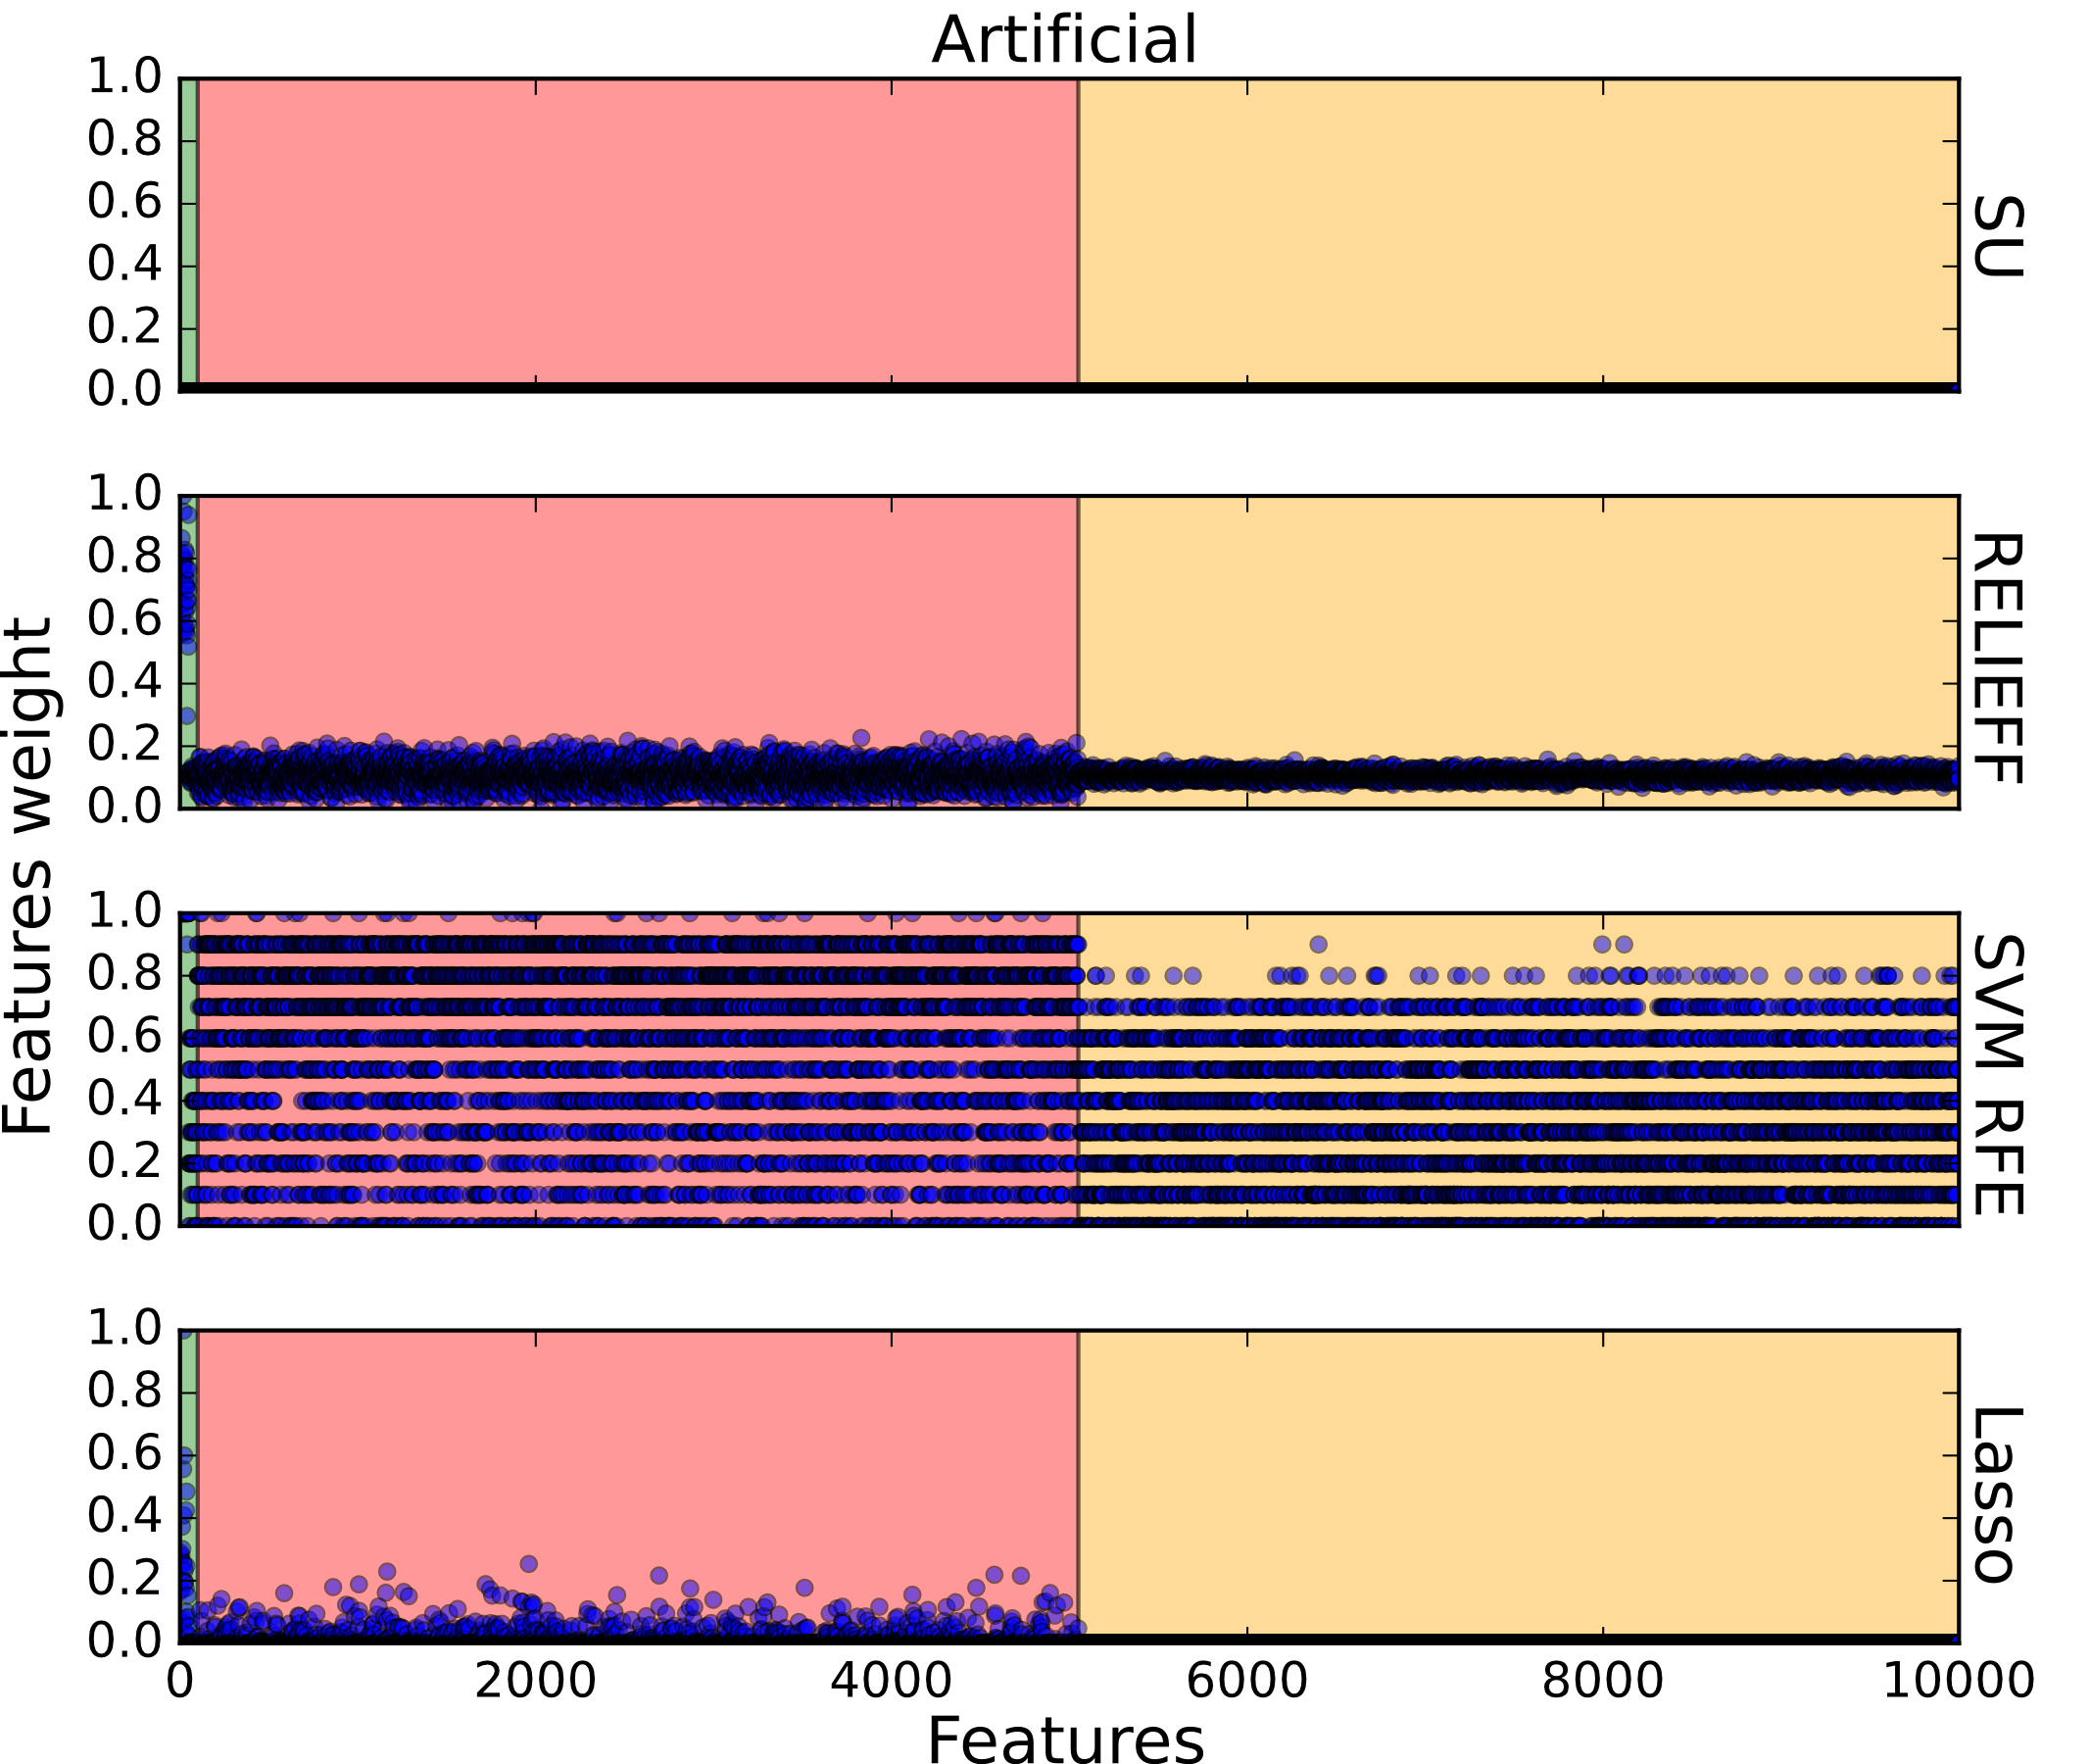
\includegraphics[width=\textwidth]{feature_weights_plot_artificial_all.png}
      \caption{Features weights for all features.}
      \label{fig:feature_weights_plot_artificial_all}
  \end{subfigure}

  \caption{The features weights for once for only the real features and once for all. In figure \ref{fig:feature_weights_plot_artificial_only_features} in the green area are the real multivariate features and in the cyan area are the real univariate features. In figure \ref{fig:feature_weights_plot_artificial_all} in the green are all real features, in the red area are the fake multivariate features and in the orange area are the fake univariate features. }
  \label{fig:feature_weights_plot_artificial}
\end{figure}
\begin{figure}[h!]
  \centering
  \caption{The histograms of the feature weights for all used feature selectors on the arcene and artificial data set.}
\end{figure}
The weights of the features can be seen in figure \ref{fig:feature_weights_plot_artificial}.
All feature selectors achieved similar results for the artificial data set except of SU. SU does not rank iall features with a zero weight which makes SU fully random on this data set. On the contrary the other feature selectors recognize parts of the inherent structure of the data. The univariate features are in general ranked lower than the multivariate features. There seems to be no diffierence in weighting between the real und fake univariate features. However the real multivariate features are ranked significantly higher than the fake multivariate features. As a consequence only multivariate features are selected. The reason why the feature selectors weight the real univariate features this low is that the univariate features do not contribute significantly to the classification. If we use only the real multivariate features with the same classification function with which the labels were created, we achieve an accuracy of $0.98$. On the other hand using the real univariate features we only achieve an accuracy of $0.52$. Therefore a feature which correlates with other significant features has significantly more impact on the classification of a data point than a uniform feature.
Furthermore the feature seletors were evaluated after how many real features they capture in the $100$ the highest weighted features. RELIEFF achieved the highest precision of $0.5$, SVM RFE achieved $0.48$, then Lasso with $0.24$ and SU with $0$.
% Acknowledgements should go at the end, before appendices and references

%\acks{I want to thank my mum}

% Manual newpage inserted to improve layout of sample file - not
% needed in general before appendices/bibliography.

\subsubsection{Different combinations of feature selectors}
The presented ensemble methods were used with all possible combinations of feature selectors. For each combination, the average of the results was taken, and the error plot corresponds to the mean of the standard deviation of each ensemble method and each dataset. While the accuracy does not change considerably with the different combinations, see figure \ref{fig:combination_accuracy}, the robustness is heavily affected by the presence or not of the feature selector Lasso as presented in the figure \ref{fig:combination_robustness}. This is due to the low robustness of the feature selector Lasso itself. On the opposite SU and RELIEFF being quite robust, their combination, with or without SVM, are the most robust.  

The methods were also compared with regards to their performance and robustness on the different combinations. However, as can be seen in figure \ref{fig:methods_results} the methods do not seems to have a great impact on the results. Therefore the choice of the combined feature selectors appears to be more important than the methods used to combine them.

\vskip 0.2in
\bibliography{references}

\newpage

\appendix
\section*{Appendix A.}
For the feature selection methods SU and RELIEFF we used the scikit-feature library from \cite{Li-etal16}.
For SVM, RFE, Lasso logistic regression we used the scikit-sklearn library from \cite{scikit-learn}
\label{app:appendixa}
\section*{Appendix B.}
\label{app:appendixb}

\begin{figure}[h!]
  \centering
    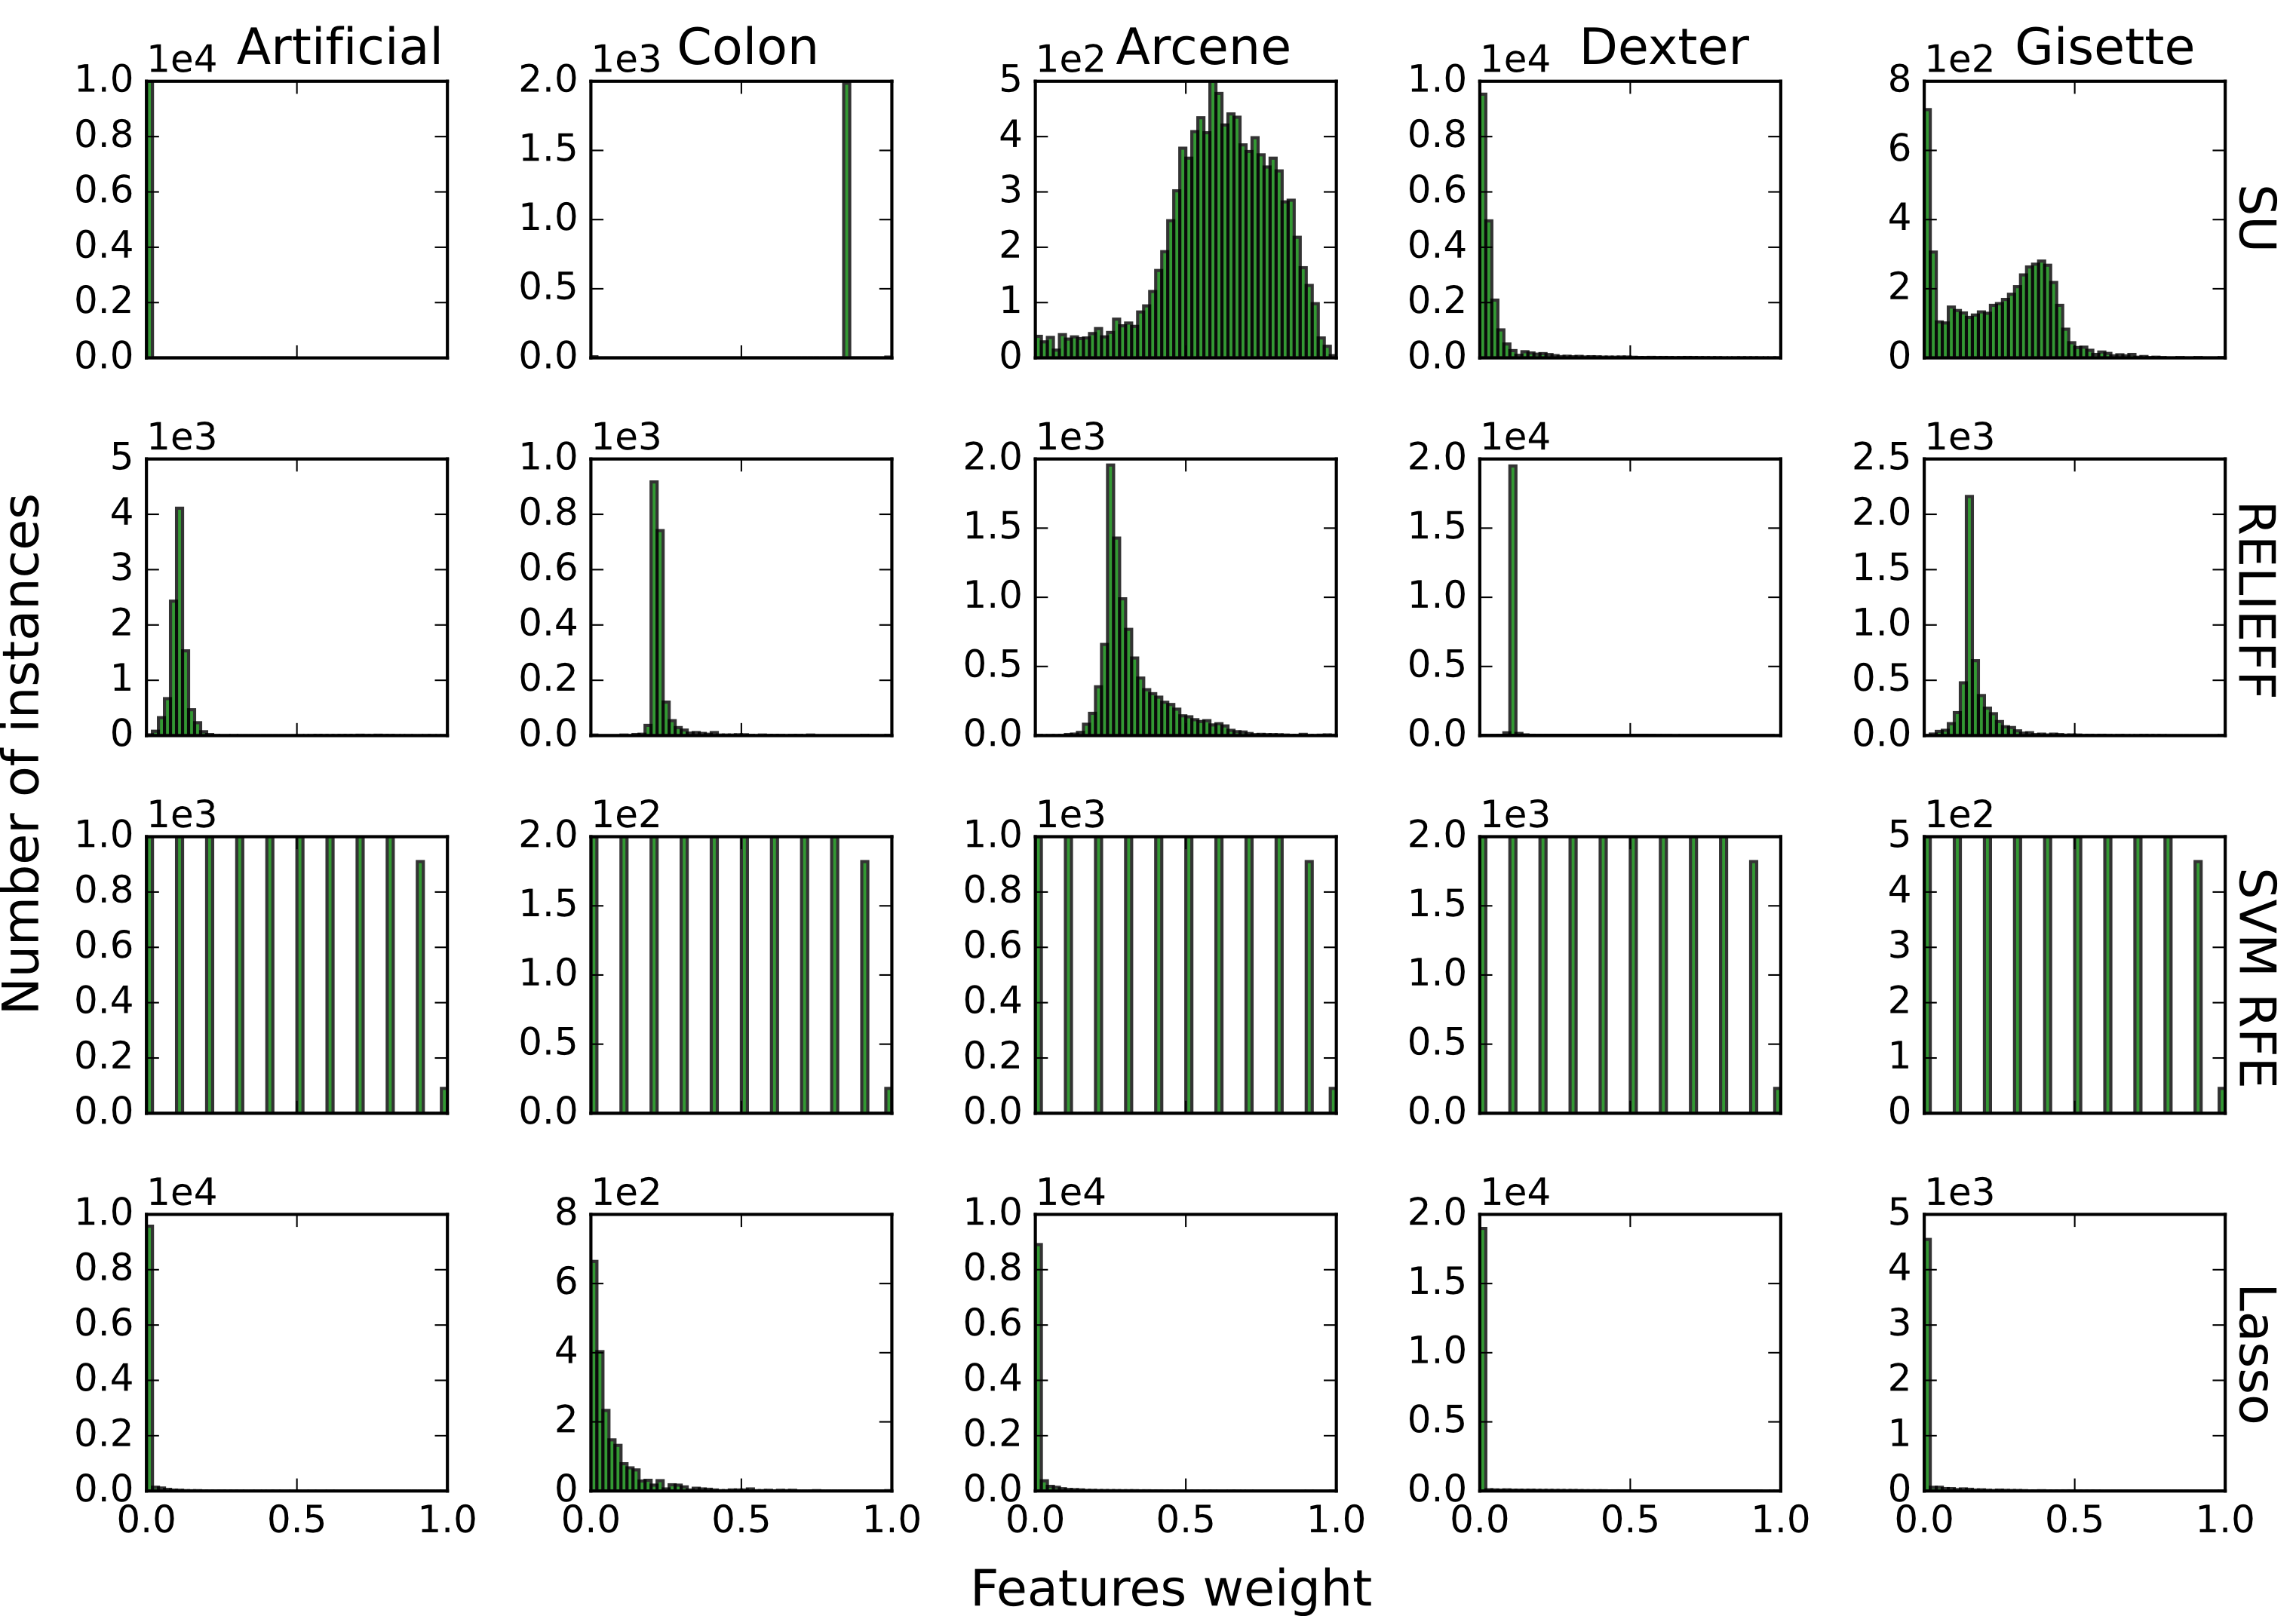
\includegraphics[width=\textwidth]{feature_weights_hist.png}
  \caption{The histogram of the feature weights for all feature selectors used for all data sets used.}
  \label{fig:feature_weights_hist}
\end{figure}

% Note: in this sample, the section number is hard-coded in. Following
% proper LaTeX conventions, it should properly be coded as a reference:


\end{document}
